\documentclass[a4]{article}
\usepackage{amssymb}
\usepackage{amsmath}
\usepackage{bm}
\usepackage{graphicx}
\usepackage{physics}
\usepackage[strings]{underscore}
\usepackage{MnSymbol}

\DeclareMathOperator*{\argmax}{argmax}
\DeclareMathOperator*{\argmin}{argmin}

%\newcommand{\bigCI}   {\mathrel{\text{\scalebox{1.07}{$\perp\mkern-10mu\perp$}}}}
%\newcommand{\bigCIneg}{\mathrel{\text{\scalebox{1.07}{$\perp\mkern-10mu\perp\mkern-18mu/$}}}}
% https://ctan.mc1.root.project-creative.net/info/symbols/comprehensive/symbols-a4.pdf

\newtheorem{defn}{Definition}

%opening
\title{ Notes on Probabilistic Graphical Models}
\author{Shoichiro Yamanishi}

\begin{document}

\maketitle

%\begin{abstract}
%\end{abstract}


\section{Overview}
This document briefly goes through some important points regarding the probabilistic graphical models.
A graphical model epresses the factoring of a joint distribution over the random variables.
Each node represent a random variable, except for a factor graph in which node is either a factor or a random variable.
A model can be programmatically drawn using Python package Daft which works with matplotlib. See \cite{daft}.

\begin{itemize}
\item Directed Acyclic Graph (Bayesian Network) : This expresses conditional dependencies among the random variables by directed edges.
\item Undirected Graph (Markov Random Field) : This expresses factoring by maximal cliques.
\item Factor Graph : This expresses the exact factoring. Any path on the graph visits factors and random variables alternatingly.
\end{itemize}

Chap.  8 of PRML \cite{bishop2007} is a good source of information.

\section{Directed Acyclic Graph (Bayesian Network)}

\subsection{Chain}
Two interesting cases: One is for a chain of 1-of-K discrete variables and the other is for gaussian distribution.
The random variables on a chain are usually latent variables.

\subsubsection{Distrete Variables Chain}
Please see Figure \ref{fig:chain_direchlet} for a chain of Direchlet distribution for latent variables
$\bm{z}_i \in \mathcal{R}^K$.
\begin{figure}[!htb]
\centering
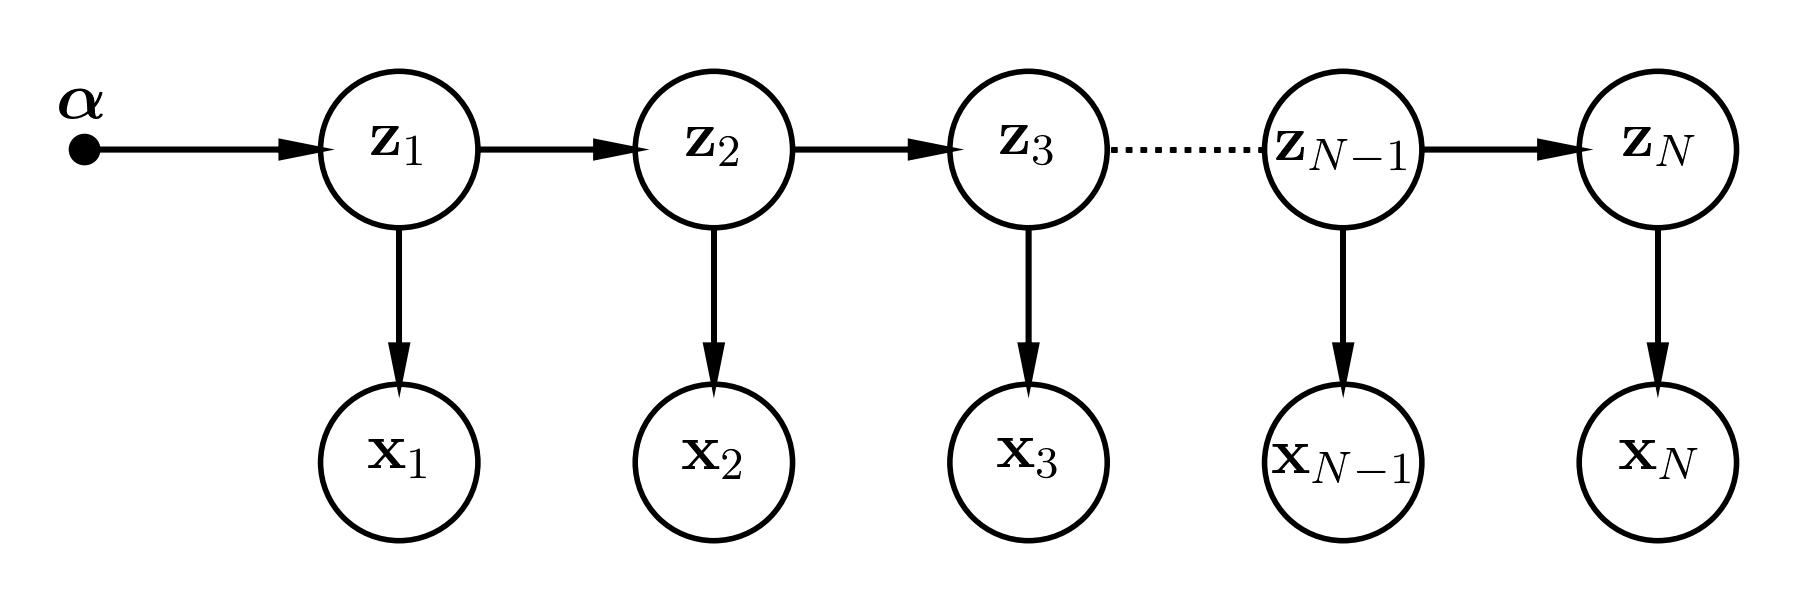
\includegraphics[width=8cm]{chain_direchlet.png}
\caption{Chain of Direchlet Distribution}
\label{fig:chain_direchlet}
\end{figure}
\begin{equation}
\begin{aligned}
p(\bm{z}_1, \bm{z}_2, \bm{z}_3, \cdots, \bm{z}_{N-1}, \bm{z}_{N} | \bm{\alpha}) &= 
p(\bm{z}_{N}|\bm{z}_{N-1})\cdots p(\bm{z}_{3}|\bm{z}_{2})p(\bm{z}_{2}|\bm{z}_{1})p(\bm{z}_{1}|\bm{\alpha})\\
&=\text{Dir}(\bm{z}_{N}|\bm{z}_{N-1})\cdots
\text{Dir}(\bm{z}_{3}|\bm{z}_{2})\text{Dir}(\bm{z}_{2}|\bm{z}_{1})\text{Dir}(\bm{z}_{1}|\bm{\alpha})\\
\end{aligned}
\end{equation}
where
$\text{Dir}(\bm{z}|\bm{\alpha}) =
\frac{\Gamma(\sum_{j=1}^K\alpha_j)}{\prod_{j=1}^K\Gamma(\alpha_j)}
\prod_{j=1}^K z_j^{\alpha_j-1}
$
 The corresponding random variables can be one-of-K variable $\bm{x}_i \in \{0,1\}^K$ such that 
$\bm{x}_i \sim \text{Mult}(\bm{x}_i| \bm{z}_i ) = \prod_{j=1}^K z_{i_j}^{x_{i_j}}$.

\subsubsection{Linear Gaussian Model}
Please see Figure \ref{fig:chain_gaussian} for a chain of Gaussian distribution for latent variables $\bm{z}_i$.
This is a conceptual model and not really useful. A useful example that includes inference to the covariance matrices
is Kalman filter described in a separate document.
\begin{figure}[!htb]
\centering
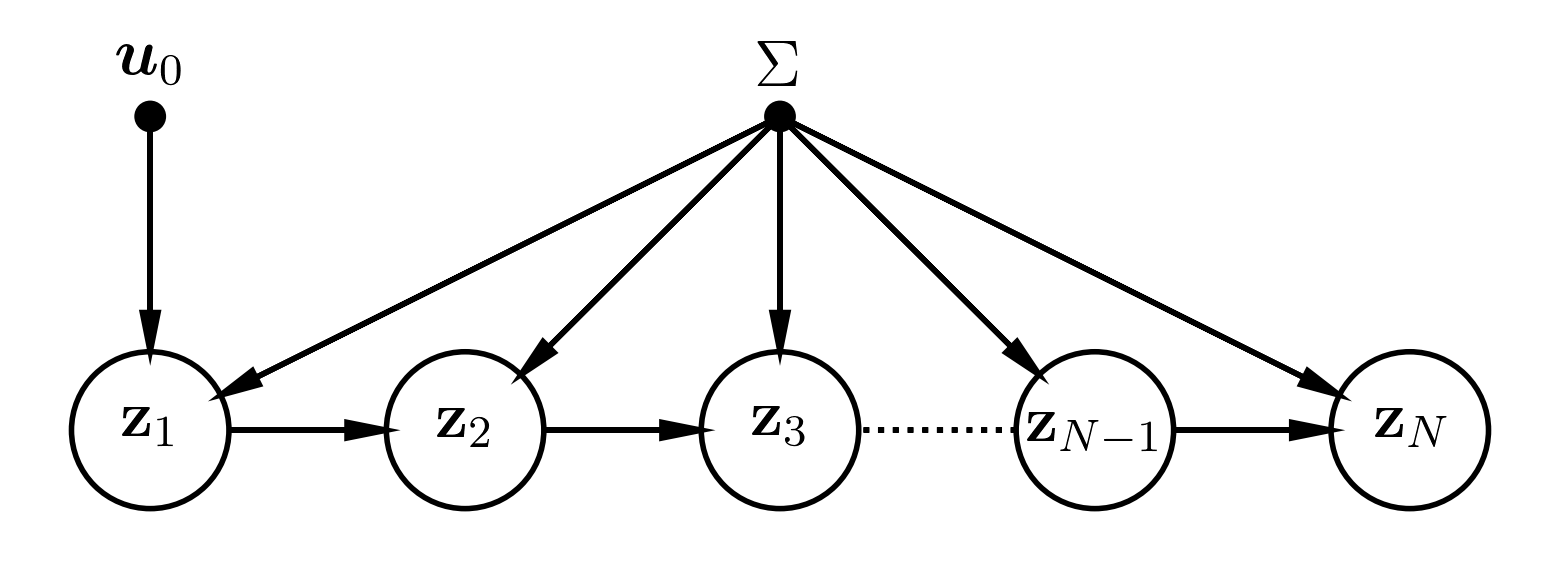
\includegraphics[width=8cm]{chain_gaussian.png}
\caption{Chain of Gaussian Distribution}
\label{fig:chain_gaussian}
\end{figure}
\begin{equation}
\begin{aligned}
p(\bm{z}_1, \bm{z}_2, \cdots, \bm{z}_{N-1}, \bm{z}_{N} | \bm{\alpha}) &= 
p(\bm{z}_{N}|\bm{z}_{N-1})\cdots p(\bm{z}_{2}|\bm{z}_{1})p(\bm{z}_{1})\\
&=\mathcal{N}(\bm{z}_{N}; \bm{u}_{N-1}(\bm{z}_{N-1}), \Sigma)\cdots
\mathcal{N}(\bm{z}_{2}; \bm{u}_{1}(\bm{z}_{1}), \Sigma)
\mathcal{N}(\bm{z}_{1}; \bm{u}_{0}, \Sigma)
\end{aligned}
\end{equation}

\subsection{Parameter Reduction}
Consider a probabbility distribution $p(y|x_1, x_2, \cdots, x_N)$
where $\bm{x}_i \in \{0,1\}^K$, $\sum_{j=1}^K x_{i_j} = 1$, i.e., $\bm{x}_i$ is a 1-of-K variable.
The possible combinations will add up to $K^N$, which could be unmanegeable.
To reduce the complexity we can use a linear combination of $\bm{x}_i$ as follows.
$p(y|x_1, x_2, \cdots, x_N, \bm{w}_0, W) = p(y| \bm{w}_0 + \sum_{i=1}^N W\bm{x}_i)$
where $\bm{w}_0 \in \mathcal{R}^K$, $W$ is a $K \cross N$ matrix.
See figure \ref{fig:param_reduction}.

\begin{figure}[!htb]
\centering
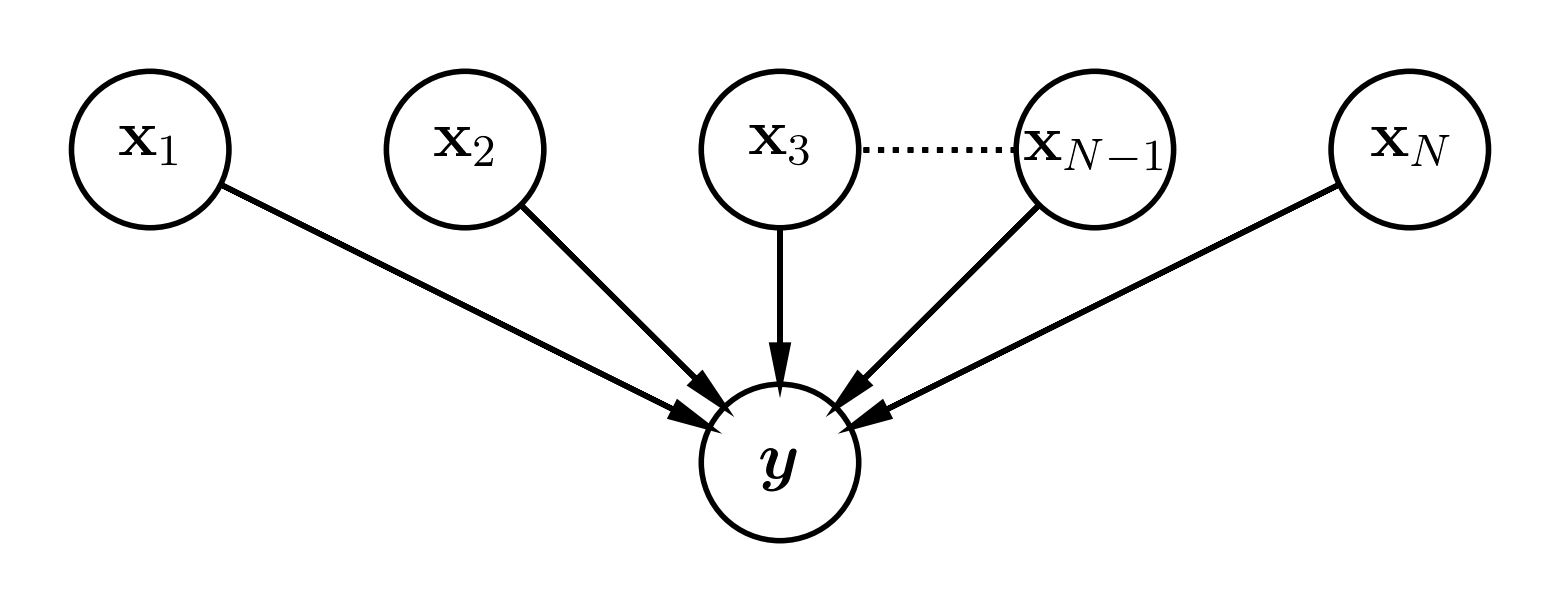
\includegraphics[width=8cm]{param_reduction.png}
\caption{Parameter Reduction}
\label{fig:param_reduction}
\end{figure}


\subsection{I.I.D. and Naive Bayes}
Consider the graphical models depicted in figure \ref{fig:iid_naive_bayes}.
This can manifest as \textit{independent and identically distributed} assumption for $N$ samples, or
\textit{Naive Bayes} model of a randam variable $\bm{x} \in \mathcal{R}^N$ with $N$ features that depends on the class $C$, where each feature is assumed to be independent of each other conditioned on $C$.
\begin{figure}[!htb]
\centering
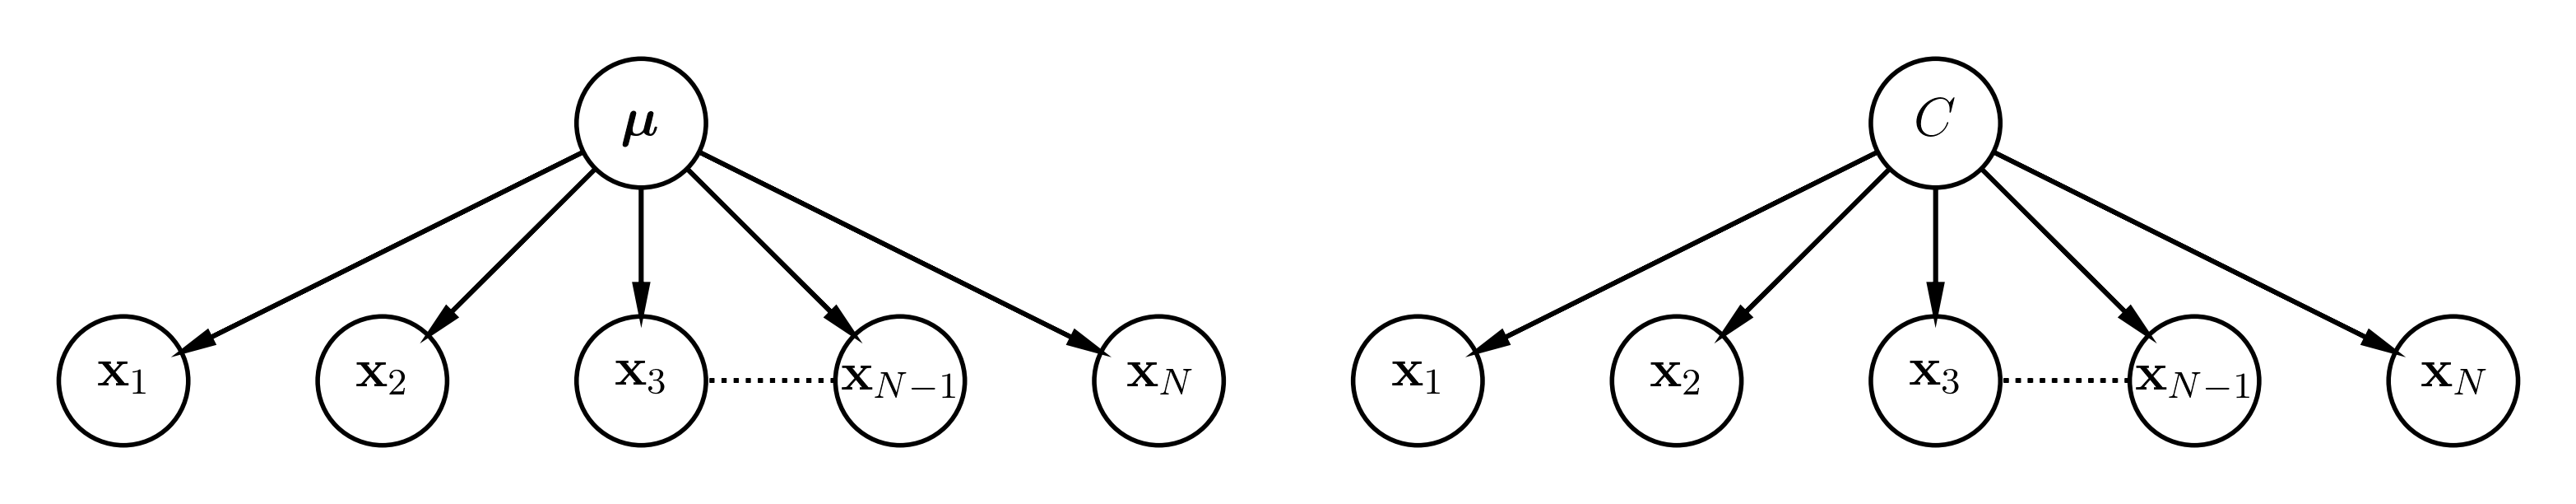
\includegraphics[width=12cm]{iid_naive_bayes.png}
\caption{I.I.D. and Naive Bayes}
\label{fig:iid_naive_bayes}
\end{figure}

\subsection{Conditional Independence, D-Separaton, and Markov Blanket}

\subsubsection{Conditional Independence}

BTW, the math symbols $\upmodels$ and $\nupmodels$ for Text are
\textit{{\textbackslash}upmodels} and \textit{{\textbackslash}nupmodels}
in the package \textit{MnSymbol}.

\begin{figure}[!htb]
\centering
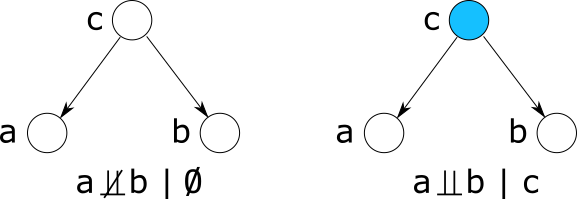
\includegraphics[width=8cm]{cond1.png}
\caption{Conditional Independence Case 1}
\label{fig:cond1}
\end{figure}

\begin{figure}[!htb]
\centering
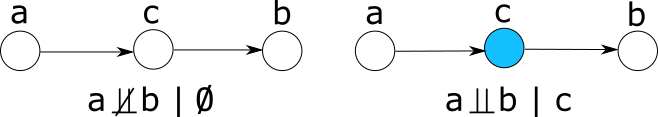
\includegraphics[width=8cm]{cond2.png}
\caption{Conditional Independence Case 2}
\label{fig:cond2}
\end{figure}

\begin{figure}[!htb]
\centering
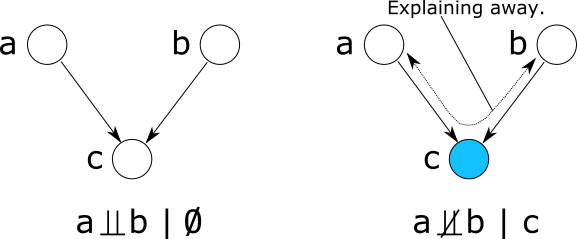
\includegraphics[width=8cm]{cond3.png}
\caption{Conditional Independence Case 3}
\label{fig:cond3}
\end{figure}

\subsubsection{D-Separation}
Let $V_s$ be a set of random variables which you want to make conditionally independent from the reset.
Given a set of observed random variables, how to determin if $V_s$ are conditionally independent from the rest?
D-Separation gives an answer. Let $G_s$ be a subgraph induced by $V_s$.
Also, Let $N^+(v)$ and $N^-(v)$ denote the in-neighbor and out-neighbor of $v$ respectively.
Then Let $N^+(G_s) = \left(\bigcup_{v \in G_s} N^+(v)\right) \setminus V(G_s)$ and
$N^-(G_s) = \left(\bigcup_{v \in G_s} N^-(v)\right) \setminus V(G_s)$ where $V(G_s)$ denotes the vertices in the graph $G_s$.
In other words, $N^+(G_s)$ is the immediate in-neighbor of $G_s$ and $N^-(G_s)$ is the immediate out-neighbor of $G_s$.
Let $D(G_s)$ be the subgraph induced by the nodes reachable from $G_s$. In other words, $D(G_s)$ is the desecendent subgraph of $G_s$.
Then in order to make $N(G_s)$ conditionally independent, the following must hold.
\begin{itemize}
\item $N^+(G_s)$ must be observed.
\item if any $v \in D(G_s)$ is observed, then $N^+(v) \setminus V(G_s)$ must be observed.
\end{itemize}
This is illustrated in figure \ref{fig:d-separation}
If the set of observed random variables meet the criteria above, then $V_s$ are conditionally independent from the rest.

\begin{figure}[!htb]
\centering
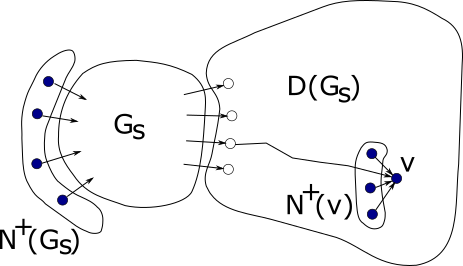
\includegraphics[width=8cm]{dseparation.png}
\caption{D-Separation}
\label{fig:d-separation}
\end{figure}

\subsubsection{Markov Blanket}
Again, let $V_s$ be a set of random variables which you want to make conditionally independent from the reset.
What other random variables must be observed to guarantee the conditional independence of $V_s$?
Markov Blanket gives an anser.
Please see figure \ref{fig:markovblanket}.
It's basically $N^+(G_s)$, $N^-(G_s)$, and its outneighbors.
\begin{figure}[!htb]
\centering
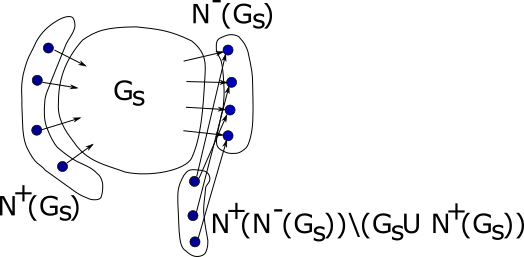
\includegraphics[width=8cm]{markovblanket.png}
\caption{D-Separation}
\label{fig:markovblanket}
\end{figure}

\section{Undirected Graph (Markov Random Field) and Belief Propagation}
We consider an exact inference called belief propagation in a tree.
There are two types to consider. One is to find a marginal distribution of a particula random variable, 
and the other is find the values for all the random variables that together maximizes the joint probability as in finding a mode in a MAP estimage.

We first consider the simple case of a chain and expand the discussion to a tree.

\subsection{Inference in a Chain : Simple Case}
Consider the joint probability of discrete random variables $\bm{x}_i \in \{0,1\}^K$, $\sum_{j=1}^K x_{i_j} = 1$,
  which is factorized into a chain as in figure \ref{fig:chain_undirected}.
\begin{figure}[!htb]
\centering
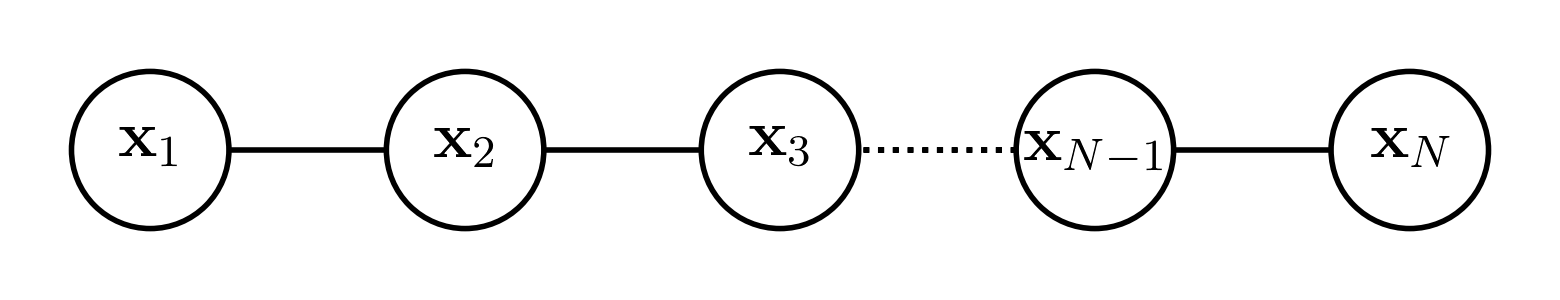
\includegraphics[width=8cm]{chain_undirected.png}
\caption{Undirected Chain}
\label{fig:chain_undirected}
\end{figure}


The joint probability is factorized into the following.
\begin{equation}
\begin{aligned}
p\left(\bm{x}_1,\bm{x}_2,\cdots, \bm{x}_{N-1},\bm{x}_{N}\right) = 
\frac{1}{Z}\phi_{1,2}(\bm{x}_1,\bm{x}_2)\phi_{2,3}(\bm{x}_2,\bm{x}_3)\cdots\phi_{N-1,N}(\bm{x}_{N-1},\bm{x}_{N})
\end{aligned}
\end{equation}
\subsubsection{Marginal distribution $p\left(\bm{x}_N\right)$}
Consider first the marginal distribution $p\left(\bm{x}_N\right)$.
\begin{equation}
\begin{aligned}
p\left(\bm{x}_{N}\right) &= 
\sum_{\bm{x}_1}\sum_{\bm{x}_2}\cdots\sum_{\bm{x}_{N-1}}
\frac{1}{Z}\phi_{1,2}(\bm{x}_1,\bm{x}_2)\phi_{2,3}(\bm{x}_2,\bm{x}_3)\cdots\phi_{N-1,N}(\bm{x}_{N-1},\bm{x}_{N})\\
&=
\frac{1}{Z}\left[
\sum_{\bm{x}_{N-1}}\phi_{N-1,N}(\bm{x}_{N-1},\bm{x}_{N})\left[
\sum_{\bm{x}_{N-2}}\phi_{N-2,N-1}(\bm{x}_{N-2},\bm{x}_{N-1})\left[
\cdots
\sum_{\bm{x}_{2}}\phi_{2,3}(\bm{x}_{2},\bm{x}_{3})\left[
\sum_{\bm{x}_{1}}\phi_{1,2}(\bm{x}_{1},\bm{x}_{2})\right]\cdots
\right]\right]\right]
\end{aligned}
\end{equation}
On the first line, there are $K^N$ terms.
On the second, I abused the notation such that each square brackets pair indicates a function of one variable.
We define the following recursive definition.
\begin{equation}
\begin{aligned}
\phi'_{i}(\bm{x}_i) = \sum_{\bm{x}_{i-1}}\phi_{i-1,i}(\bm{x}_{i-1}, \bm{x}_{i})\phi'_{i-1}(\bm{x}_{i-1})
\end{aligned}
\end{equation}
Evaluation of each of $K$ elements of $\phi'_i(\bm{x}_{i})$ takes 
takes $K$ evaluations of $\phi(\bm{x}_{i-1},\bm{x}_{i})$, 
$K$ multiplications, and $K-1$ additions. Hence the construction of one $\phi'_i(\bm{x}_{i})$ is $O(K^2)$.

Then $p(\bm{x}_N)$ is constructed sequencially by evaluating from $\phi'_1(\bm{x}_{2})$ up to $\phi'_1(\bm{x}_{N})$
as follows.
\begin{equation}
\begin{aligned}
p\left(\bm{x}_{N}\right) &= 
\frac{1}{Z}\left[
\sum_{\bm{x}_{N-1}}\phi_{N-1,N}(\bm{x}_{N-1},\bm{x}_{N})\left[
\sum_{\bm{x}_{N-2}}\phi_{N-2,N-1}(\bm{x}_{N-2},\bm{x}_{N-1})\left[
\cdots
\sum_{\bm{x}_{2}}\phi_{2,3}(\bm{x}_{2},\bm{x}_{3})\left[
\sum_{\bm{x}_{1}}\phi_{1,2}(\bm{x}_{1},\bm{x}_{2})\right]\cdots
\right]\right]\right]\\
&=
\frac{1}{Z}\left[
\sum_{\bm{x}_{N-1}}\phi_{N-1,N}(\bm{x}_{N-1},\bm{x}_{N})\left[
\sum_{\bm{x}_{N-2}}\phi_{N-2,N-1}(\bm{x}_{N-2},\bm{x}_{N-1})\left[
\cdots
\sum_{\bm{x}_{2}}\phi_{2,3}(\bm{x}_{2},\bm{x}_{3})\phi'_2(\bm{x}_2)
\right]\right]\right]\\
&=
\frac{1}{Z}\left[
\sum_{\bm{x}_{N-1}}\phi_{N-1,N}(\bm{x}_{N-1},\bm{x}_{N})\left[
\sum_{\bm{x}_{N-2}}\phi_{N-2,N-1}(\bm{x}_{N-2},\bm{x}_{N-1})\left[
\cdots
\phi'_3(\bm{x}_3)
\right]\right]\right]\\
&=
\frac{1}{Z}\left[
\sum_{\bm{x}_{N-1}}\phi_{N-1,N}(\bm{x}_{N-1},\bm{x}_{N})\left[
\sum_{\bm{x}_{N-2}}\phi_{N-2,N-1}(\bm{x}_{N-2},\bm{x}_{N-1})\phi'_{N-2}(\bm{x}_{N-2})
\right]\right]\\
&=
\frac{1}{Z}\left[
\sum_{\bm{x}_{N-1}}\phi_{N-1,N}(\bm{x}_{N-1},\bm{x}_{N})\phi'_{N-1}(\bm{x}_{N-1})
\right]\\
&=
\frac{1}{Z}\phi'_N(\bm{x}_{N})
\end{aligned}
\end{equation}
This derivation can be viewed as a message passing from $\bm{x}_2$ up to $\bm{x}_N$ with the message defined by 
$\phi'_{i}(\bm{x}_{i})$. This is the simplest form of belief propagation.

Please note that $Z = \sum_{\bm{x}_N}\phi'_N(\bm{x}_{N})$.
Overall the complexity of finding  $p(\bm{x}_{N})$ is $O(NK^2)$.

\subsubsection{Finding a Mode : $\argmax\{p\left(\bm{x}_1,\bm{x}_2,\cdots, \bm{x}_{N-1},\bm{x}_{N}\right)\}$ for MAP etc}
Now we want to find the values for each random variables that maximizes the joint probability. This occurs in a MAP estimate, where
you want to get the highest mode of the probability distribution.
Here we define an operation called $amax$ to be a combined operation of max and argmax. I.e., it stores both the maximum value
as well as the element that holds the maximum value.

\begin{equation}
\begin{aligned}
(p^*, \bm{x}^*_1, \bm{x}^*_2, \cdots, \bm{x}^*_N)
&= 
\underset{\bm{x}_1, \bm{x}_2, \cdots, \bm{x}_N}{\mathrm{amax}}\left\{
p\left(\bm{x}_1,\bm{x}_2,\cdots, \bm{x}_{N-1},\bm{x}_{N}\right)\right\}\\
&= 
\underset{\bm{x}_1, \bm{x}_2, \cdots, \bm{x}_N}{\mathrm{amax}}\left\{
\frac{1}{Z}\phi_{1,2}(\bm{x}_1,\bm{x}_2)\phi_{2,3}(\bm{x}_2,\bm{x}_3)\cdots\phi_{N-1,N}(\bm{x}_{N-1},\bm{x}_{N})
\right\}\\
\end{aligned}
\end{equation}

We can exploit the chain structure to ditribute the $amax$ operation as follows.


\begin{equation}
\begin{aligned}
&\:\:
\underset{\bm{x}_1, \bm{x}_2, \cdots, \bm{x}_N}{\mathrm{amax}}\left\{
    \frac{1}{Z}\phi_{1,2}(\bm{x}_1,\bm{x}_2)\phi_{2,3}(\bm{x}_2,\bm{x}_3)\cdots\phi_{N-1,N}(\bm{x}_{N-1},\bm{x}_{N})
\right\}\\
&=
\underset{\bm{x}_1}{\mathrm{amax}}\left\{
\underset{\bm{x}_2}{\mathrm{amax}}\left\{
\phi_{1,2}(\bm{x}_1,\bm{x}_2)
\underset{\bm{x}_3}{\mathrm{amax}}\left\{
\phi_{2,3}(\bm{x}_2,\bm{x}_3)
\cdots
\underset{\bm{x}_N}{\mathrm{amax}}\left\{
\phi_{N-1,N}(\bm{x}_{N-1},\bm{x}_{N})
\right\}\cdots
\right\}
\right\}
\right\}\\
\end{aligned}
\end{equation}
where I abused the notation of $\underset{\bm{x}_{i-1}}{\mathrm{amax}}\left\{\right\}$ be
a function of $\bm{x}_i$.

We define the following recursive definition.
\begin{equation}
\begin{aligned}
\phi'_{i-1}(\bm{x}_{i-1}) = 
\underset{\bm{x}_{i}}{\mathrm{amax}}\left\{
\phi_{i-1,i}(\bm{x}_{i-1}, \bm{x}_{i})\phi'_{i-1}(\bm{x}_{i-1})\right\}
\end{aligned}
\end{equation}
Evaluation of each of $K$ elements of $\phi'_{i-1}(\bm{x}_{i-1})$ takes 
takes $K$ evaluations of $\phi(\bm{x}_{i-1},\bm{x}_{i})$ and 
$K$ comparisons. Hence the construction of one $\phi'_{i-1}(\bm{x}_{i-1})$ is $O(K^2)$.
Then,
\begin{equation}
\begin{aligned}
&\:\:
\underset{\bm{x}_1}{\mathrm{amax}}\left\{
\underset{\bm{x}_2}{\mathrm{amax}}\left\{
\phi_{1,2}(\bm{x}_1,\bm{x}_2)
\underset{\bm{x}_3}{\mathrm{amax}}\left\{
\phi_{2,3}(\bm{x}_2,\bm{x}_3)
\cdots
\underset{\bm{x}_N}{\mathrm{amax}}\left\{
\phi_{N-1,N}(\bm{x}_{N-1},\bm{x}_{N})
\right\}\cdots
\right\}
\right\}
\right\}\\
&=
\underset{\bm{x}_1}{\mathrm{amax}}\left\{
\underset{\bm{x}_2}{\mathrm{amax}}\left\{
\phi_{1,2}(\bm{x}_1,\bm{x}_2)
\underset{\bm{x}_3}{\mathrm{amax}}\left\{
\phi_{2,3}(\bm{x}_2,\bm{x}_3)
\cdots
\phi'_{N-1}(\bm{x}_{N-1})
\cdots
\right\}
\right\}
\right\}\\
&=
\underset{\bm{x}_1}{\mathrm{amax}}\left\{
\underset{\bm{x}_2}{\mathrm{amax}}\left\{
\phi_{1,2}(\bm{x}_1,\bm{x}_2)
\phi'_{2}(\bm{x}_{2})
\right\}
\right\}\\
&=
\underset{\bm{x}_1}{\mathrm{amax}}\left\{
\phi'_{1}(\bm{x}_{1})
\right\}\\
&=
(p^*, \bm{x}^*_1)
\end{aligned}
\end{equation}

This derivation can be viewed as a message passing from $\bm{x}_{N-1}$ up to $\bm{x}_1$ with the message defined by 
$\phi'_{i}(\bm{x}_{i})$.
To obtain $(\bm{x}^*_2, \cdots, \bm{x}^*_N)$, we can back track the operation from $\bm{x}_1$ to $\bm{x}_{N-1}$.
Overall the complexity of finding  $p(\bm{x}_{N})$ is $O(NK^2)$.

\subsection{Inference in a Tree}
We extend the idea described in the chain to trees.
There are two types of extensions in the factor graph.
\begin{itemize}
\item One factor can take more than two random variables.
\item One variable can be associated to more than two factors.
\end{itemize}
In order to accommodate those extensions, we define the recursive relation in two phases.
Please see figure \ref{fig:tree}.

\begin{figure}[!htb]
\centering
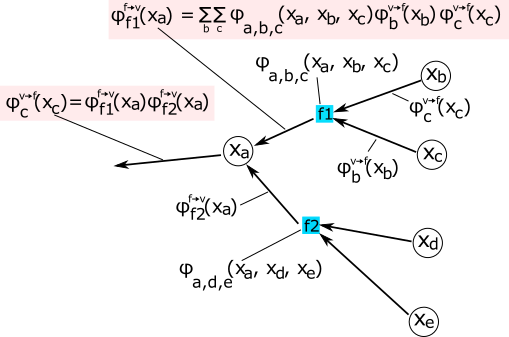
\includegraphics[width=8cm]{tree.png}
\caption{Propagation in a Tree}
\label{fig:tree}
\end{figure}

We have to nominate one random variable node $\bm{x}_{root}$ in the factor graph as the root, and
form a rooted oriented tree by orienting the edges from the root toward leaves. Such a tree is unique up to the edge
orientation. In case of marginalization, $\bm{x}_{root}$ is the random variable for which, the rest of the random variables
are marginalized to obtain $p(\bm{x}_{root})$.

$\phi^{f\rightarrow v}_{\bm{f}}(\bm{x})$ is from a factor to a variable, and
$\phi^{v\rightarrow f}_{\bm{x}}(\bm{x})$ is from a variable to a factor.

$\phi^{f\rightarrow v}_{\bm{f}_a}(\bm{x}_i)$ represent the subtree under $\bm{f}_a$ as a function of $\bm{x}_i$.
$\phi^{v\rightarrow f}_{\bm{x}_i}(\bm{x}_i)$ represent the subtree under $\bm{x}_i$ as a function of $\bm{x}_i$, i.e., 
$$\phi^{v\rightarrow f}_{\bm{x}_i}(\bm{x}_i) = \prod_{\bm{f}_j \in N^-(\bm{x}_i)}\phi^{f\rightarrow v}_{\bm{f}_j}(\bm{x}_i)$$
Now, $\phi^{f\rightarrow v}_{\bm{f}}(\bm{x}_a)$ is defined as a marginalization or maximization of 
$\phi_{\bm{x}_{i1},\bm{x}_{i2},\cdots, \bm{x}_{iL}}(\bm{x}_{i1},\bm{x}_{i2},\cdots, \bm{x}_{iL})$
where $\bm{x}_a \in \{\bm{x}_{i1},\bm{x}_{i2},\cdots, \bm{x}_{iL}\}$.
Then 
\begin{equation}
\begin{aligned}
\phi^{f\rightarrow v}_{\bm{x}_a}(\bm{x}_a)
=
\sum_{\{\bm{x}_{i1},\bm{x}_{i2},\cdots, \bm{x}_{iL}\}\setminus\bm{x}_a}\left(
    \phi_{\bm{x}_{i1},\bm{x}_{i2},\cdots, \bm{x}_{iL}}(\bm{x}_{i1},\bm{x}_{i2},\cdots, \bm{x}_{iL})
    \prod_{\bm{x}_b}^{\{\bm{x}_{i1},\bm{x}_{i2},\cdots, \bm{x}_{iL}\}\setminus\bm{x}_a}\left(
        \phi^{v\rightarrow f}_{\bm{x}_b}(\bm{x}_b)
    \right)
\right)
\end{aligned}
\end{equation}
or, 
\begin{equation}
\begin{aligned}
\phi^{f\rightarrow v}_{\bm{x}_a}(\bm{x}_a)
=
\underset{\{\bm{x}_{i1},\bm{x}_{i2},\cdots, \bm{x}_{iL}\}\setminus\bm{x}_a}{\mathrm{amax}}
\left\{
    \phi_{\bm{x}_{i1},\bm{x}_{i2},\cdots, \bm{x}_{iL}}(\bm{x}_{i1},\bm{x}_{i2},\cdots, \bm{x}_{iL})
    \prod_{\bm{x}_b}^{\{\bm{x}_{i1},\bm{x}_{i2},\cdots, \bm{x}_{iL}\}\setminus\bm{x}_a}\left(
        \phi^{v\rightarrow f}_{\bm{x}_b}(\bm{x}_b)
    \right)
\right\}
\end{aligned}
\end{equation}

\subsection{Inference in a Grid}
We can't use a belief propagation if the graph contains a cycle.
If we force a belief propagation to such a graph and assume the propagation to converge,
then it is called \textit{loopy belief propagation}.

Assume the latent variables are discrete, i.e. $\bm{x}_i = \{0,1\}^K$, $\sum_{j=1}^K x_{i_j} = 1$
and the joint probability is represented as follows.
\begin{equation}
\begin{aligned}
    p(\bm{x}_1, \bm{x}_2, \cdots, \bm{x}_N, \bm{z}_1, \bm{z}_2, \cdots, \bm{z}_N)
&= 
    \prod_{i=1}^N p(\bm{x}_i|\bm{z}_i) p(\bm{z}_1, \bm{z}_2, \cdots, \bm{z}_N)\\
&= 
    \prod_{i=1}^N p(\bm{x}_i|\bm{z}_i) \prod_{\{u,v\}\in \mathcal{C}} p(\bm{z}_u, \bm{z}_v)\\
&= 
    \prod_{i=1}^N \text{Mult}(\bm{x}_i|\bm{z}_i) 
    \prod_{\{u,v\}\in \mathcal{C}} \frac{1}{Z_{\{u,v\}}}\exp\left(-\phi\left(\bm{z}_u, \bm{z}_v\right)\right)\\
&= 
    \prod_{i=1}^N \prod_{j=1}^K (z_{i_j}^{x_{i_j}})
    \frac{1}{Z_w}\exp\left( - \sum_{\{u,v\}\in \mathcal{C}} \phi\left(\bm{z}_u, \bm{z}_v\right)\right)\\
&= 
    \frac{1}{Z}\exp\left(
    \sum_{i=1}^N \sum_{j=1}^K x_{i_j}\ln({z_{i_j}})
     - \sum_{\{u,v\}\in \mathcal{C}} \phi\left(\bm{z}_u, \bm{z}_v\right)\right)\\
&= 
    \frac{1}{Z}\exp\left(
    \sum_{i=1}^N U_i(z_i)
     - \sum_{\{u,v\}\in \mathcal{C}} P_{u,v}\left(\bm{z}_u, \bm{z}_v\right)\right)\\
\end{aligned}
\end{equation}
where $\mathcal{C}$ is the set of edges in the grid.
Please see figure \ref{fig:grid_generative}
\begin{figure}[!htb]
\centering
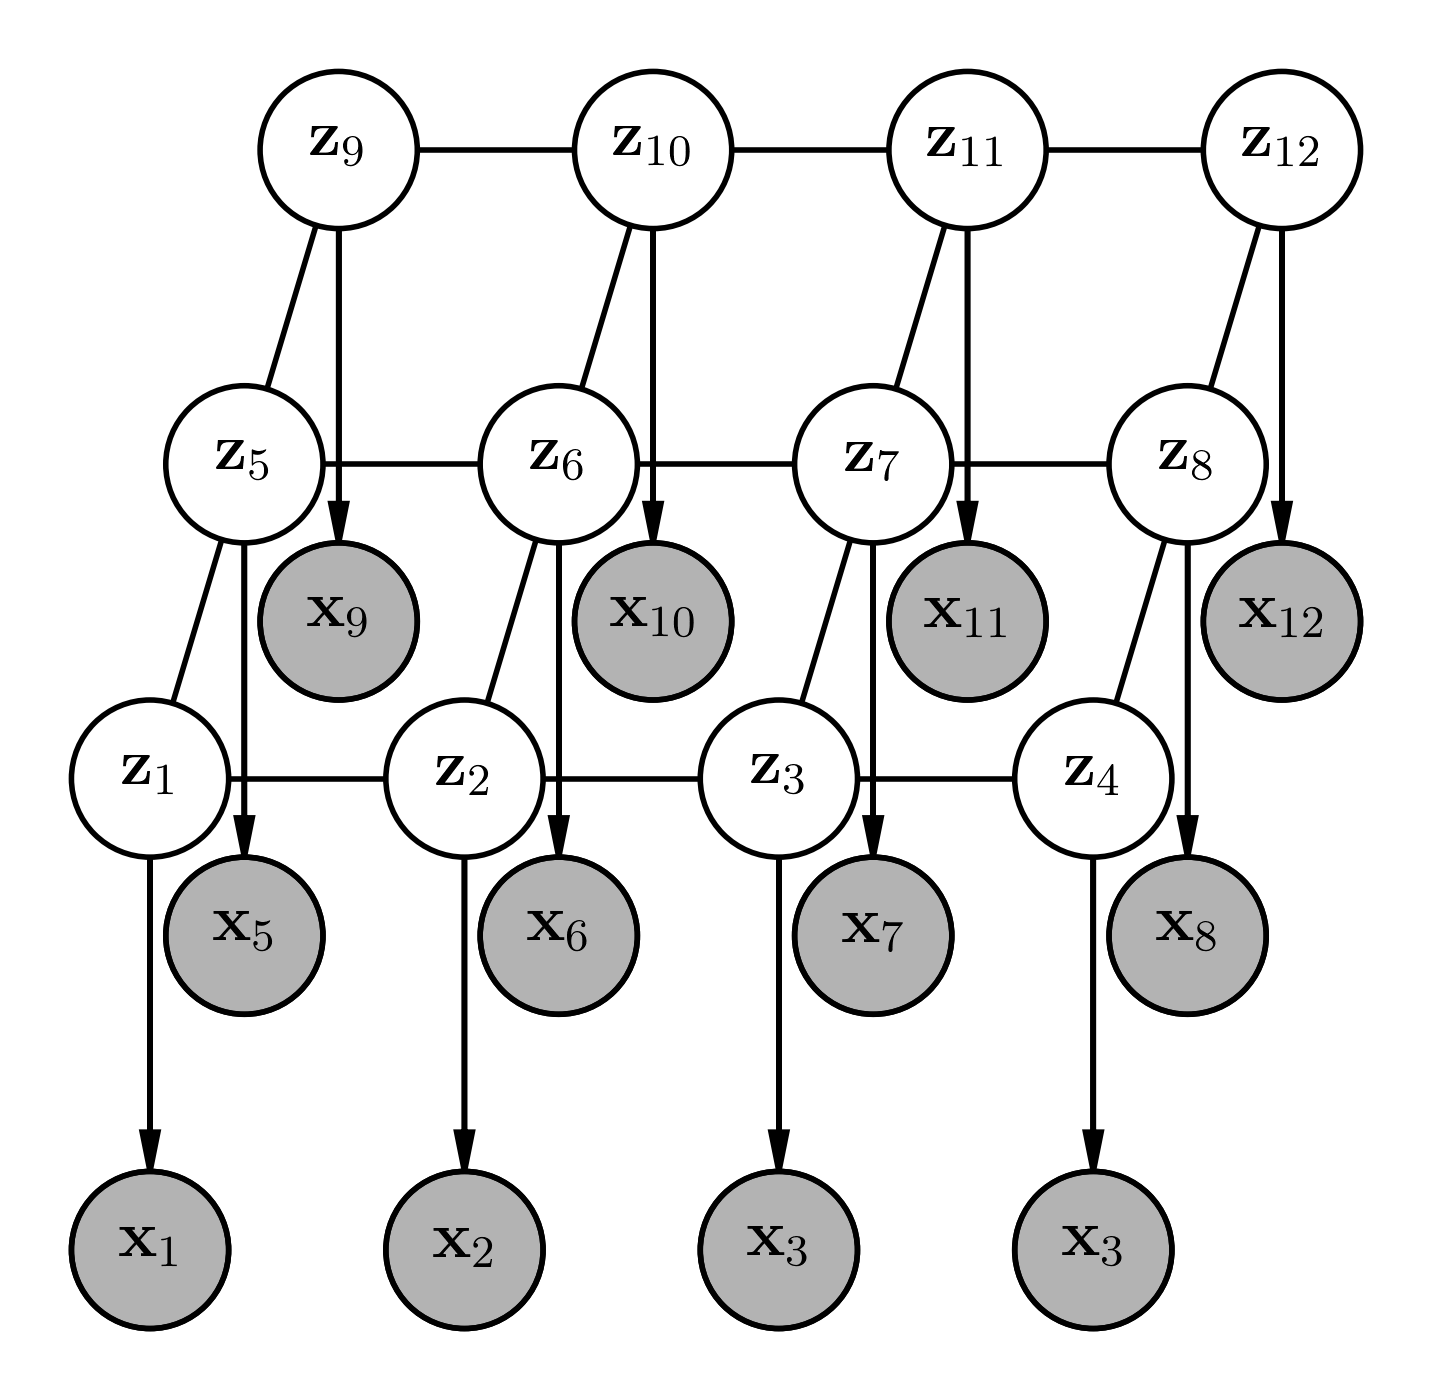
\includegraphics[width=6cm]{grid_generative.png}
\caption{Generative Grid}
\label{fig:grid_generative}
\end{figure}


After observing $(\bm{x}_1, \bm{x}_2, \cdots, \bm{x}_N)$, the posterior will be:
\begin{equation}
\begin{aligned}
    p( \bm{z}_1, \bm{z}_2, \cdots, \bm{z}_N | \bm{x}_1, \bm{x}_2, \cdots, \bm{x}_N )
&= 
    \frac{p( \bm{x}_1, \bm{x}_2, \cdots, \bm{x}_N , \bm{z}_1, \bm{z}_2, \cdots, \bm{z}_N ) }
         {p( \bm{x}_1, \bm{x}_2, \cdots, \bm{x}_N ) }\\
&\propto
    p( \bm{x}_1, \bm{x}_2, \cdots, \bm{x}_N , \bm{z}_1, \bm{z}_2, \cdots, \bm{z}_N )\\
&= 
    \frac{1}{Z}\exp\left(
    \sum_{i=1}^N U_i(z_i)
     - \sum_{\{u,v\}\in \mathcal{C}} P_{u,v}\left(\bm{z}_u, \bm{z}_v\right)\right)\\
\end{aligned}
\end{equation}

Then the MAP estimate will be:
\begin{equation}
\begin{aligned}
\underset{\bm{z}_1, \bm{z}_2, \cdots, \bm{z}_N}{\mathrm{argmax}}
\left\{
    p(\bm{x}_1, \bm{x}_2, \cdots, \bm{x}_N, \bm{z}_1, \bm{z}_2, \cdots, \bm{z}_N)
\right\}
&=
\underset{\bm{z}_1, \bm{z}_2, \cdots, \bm{z}_N}{\mathrm{argmax}}
\left\{
    \sum_{i=1}^N U_i(z_i)
     - \sum_{\{u,v\}\in \mathcal{C}} P_{u,v}\left(\bm{z}_u, \bm{z}_v\right)
\right\}\\
\end{aligned}
\end{equation}

If you want a MAP estimate, then we can use a max-flow min-cut paradigm, but it will be inpractical if $K$ is large, as 
you have to form a graph whose number of nodes is $K+1$ times the number of latent variables, and between two latent variables
there are $2K + K^2$ edges as a acomplete bipartite graph.
Please see section 12.2 and 12.3 of \cite{prince_2012}.

The same technique can be applied for a model in conditional random field as in figure \ref{fig:grid_crf}.
The probability distribution is formulated as follows.
\begin{equation}
\begin{aligned}
    p(\bm{x}_1, \bm{x}_2, \cdots, \bm{x}_N, \bm{z}_1, \bm{z}_2, \cdots, \bm{z}_N)
&=
    \frac{1}{Z}\exp\left(
     - \sum_{\{u,v\}\in \mathcal{C}} \phi\left(\bm{z}_u, \bm{z}_v\right)
     - \sum_{i=1}^N \eta\left(\bm{x}_i, \bm{z}_i\right)\right)\\
\end{aligned}
\end{equation}


\begin{figure}[!htb]
\centering
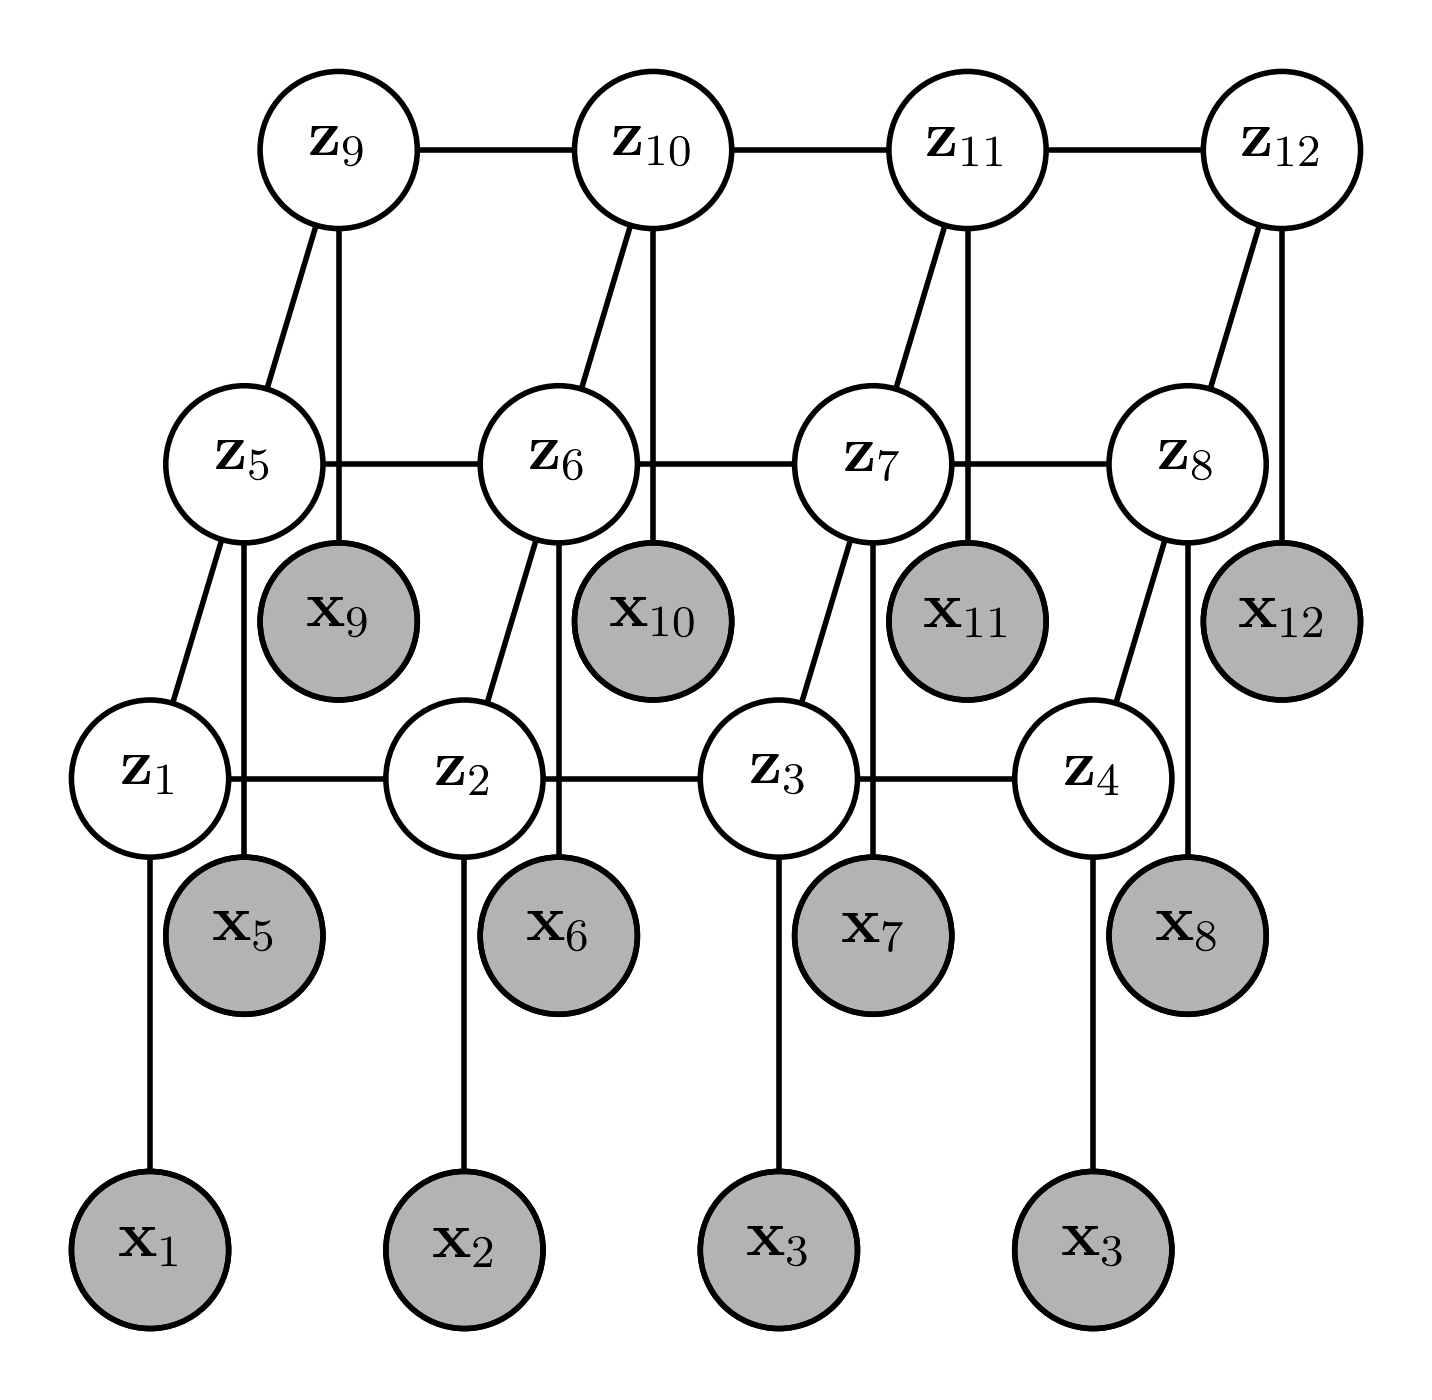
\includegraphics[width=6cm]{grid_crf.png}
\caption{Conditional Random Field Grid}
\label{fig:grid_crf}
\end{figure}


\bibliography{graphicalmodels.bib}{}
\bibliographystyle{plain}

\end{document}
